\section{Zielsetzung}
In den beiden folgenden Experimenten soll die Ablenkung von Elektronen im elektrischen und magnetischen Feld untersucht werden. Außerdem soll die Stärke des Erdmagnetfeldes bestimmt werden.

\section{Theoretische Grundlage}
\label{sec:Theorie}
\subsection{Aufbau der Kathodenstrahlröhre}
Die beiden Versuche werden in einem Hochvakuum durchgeführt, da die Elektronen sonst mit den Luftmolekülen wechselwirken würden. Dazu wird die Kathodenstrahlröhre (Braunsche Röhre) verwendet. Diese besteht aus drei Hauptkomponenten: der Elektronenkanone, einem Ablenksystem und einem Nachweissystem.\\
\textbf{Die Elektronenkanone:} \\
Die Elektronenkanone erzeugt freie Elektronen durch Glühemission und beschleunigt diese. Da zu wird ein Kathode indirekt beheizt. Diese wird von dem Wehnelt-Zylinder umgeben welcher die Intensität des Elektronenstrahls steuert. Die Elektronen werden durch einen nachfolgenden Anodenring beschleunigt. Danach werden die beschleunigten Elektronen Fokussiert.
\textbf{Das Ablenksystem:} \\
Das Ablenksystem besteht aus zwei, zueinander parrallelen Kondensatorplatten, welche ein annähernd homogenes elektrisches Feld erzeugen in dem die Elektronen Abgelenkt werden. Sollen die Elektronen in eine weitere Richtung abgelenkt werden wird ein weiteres Plattenpaar um 90 Grad versetzt eingebaut.
\textbf{Das Nachweissystem:} \\
Das Nachweissystem visualisiert den auftrefenden Elektronenstrahl.\\
In der nachfolgenden Abbildung wird der Sachverhalt verdeutlicht.

\begin{figure}[H]
	\centering
	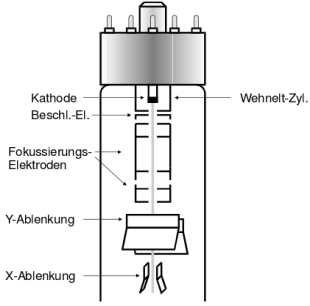
\includegraphics[height=7cm]{picture/Kathodenstrahlroehre.PNG}
	\caption{Schematischer Aufbau einer Kathodenstrahlröhre}
	\label{fig:Kathode}
\end{figure}

\subsection{Ablenkung von Elektronen im E-Feld}















\subsection{Fehlerrechnung}
